\documentclass[Nike]{tuberlinbeamer}

\usepackage[ngerman]{babel}  % 'babel' muss geladen werden
\usepackage[utf8]{inputenc}  % optional, aber empfehlenswert
\usepackage[square,numbers]{natbib}
\usepackage[]{algorithm2e}
\usepackage{caption}
\captionsetup[figure]{labelformat=empty}

% Die ueblichen Angaben
\title{Recurrent Neural Networks}
\subtitle{Machine Learning Group}
\author[SS.2018 Deep Neural Networks]{Dr. Gr\'egoire Montavon}
\institute{Technische Universität Berlin}

% Eigenes Logo einfuegen:
\renewcommand{\pathtomylogo}{ida_logo}
\newcommand{\x}[0]{\boldsymbol{x}}
\newcommand{\pvec}[1]{\boldsymbol{#1}}
\newcommand{\ppartial}[2]{\frac{\partial #1}{\partial #2}}

\begin{document}

\begin{frame}
\maketitle
\end{frame}


\begin{frame}{Outline}
\tableofcontents
\end{frame}

\section{Recurrent Neural Networks}
\subsection{Overview \& Applications}
\begin{frame}{What are Recurrent Neural Networks (RNNs)?}

\only<1>{
\vspace*{\fill}
	\begin{figure}[h]
	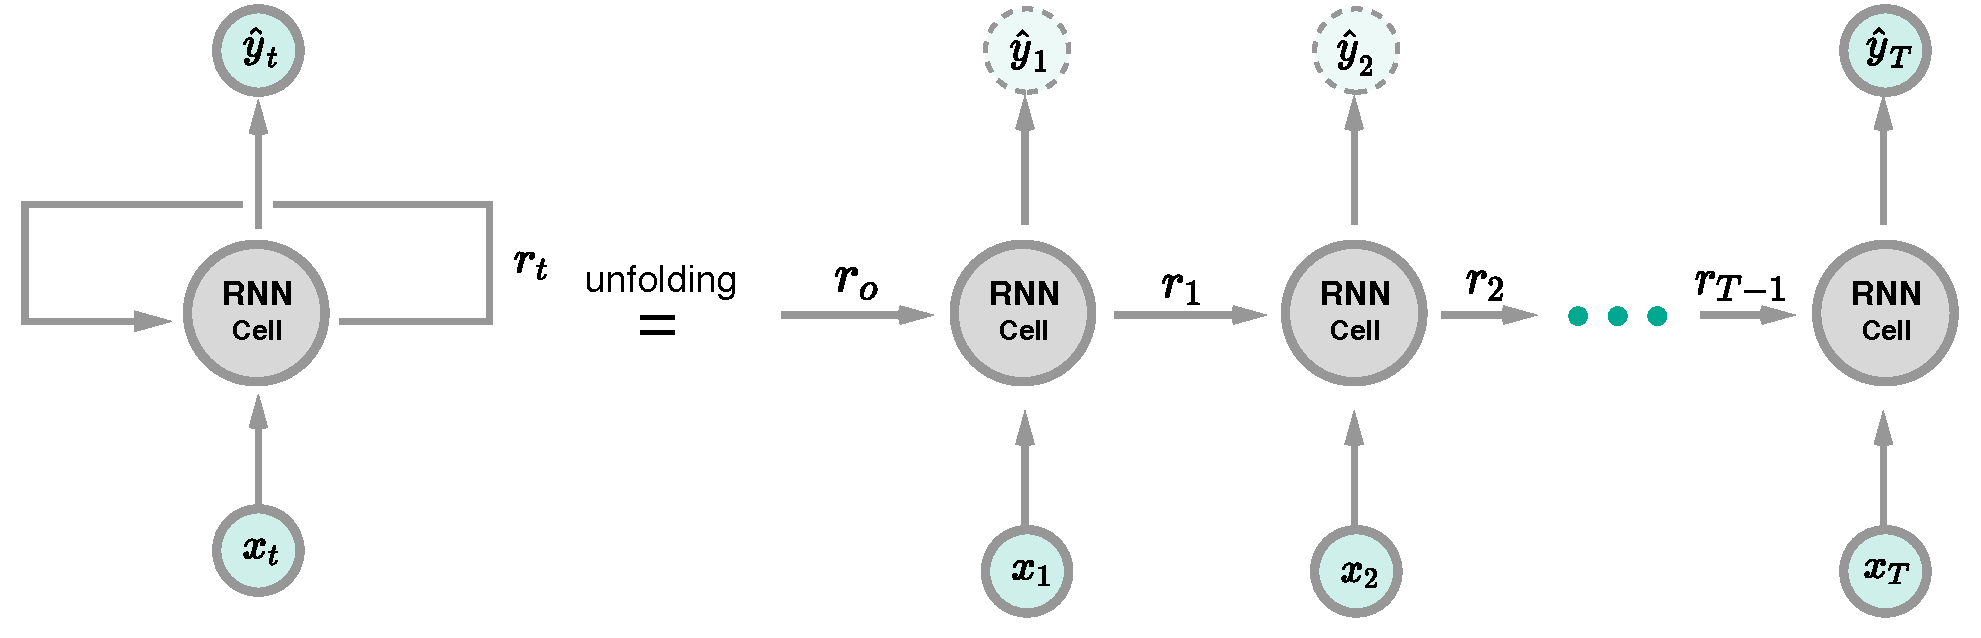
\includegraphics [width=0.8\textwidth]{figures/rnn_unfold}
	\end{figure}	
\vspace*{\fill}
}
\only<2->{
Example Applications
	\only<2>{
			\vspace*{\fill}
			\begin{figure}[h]
				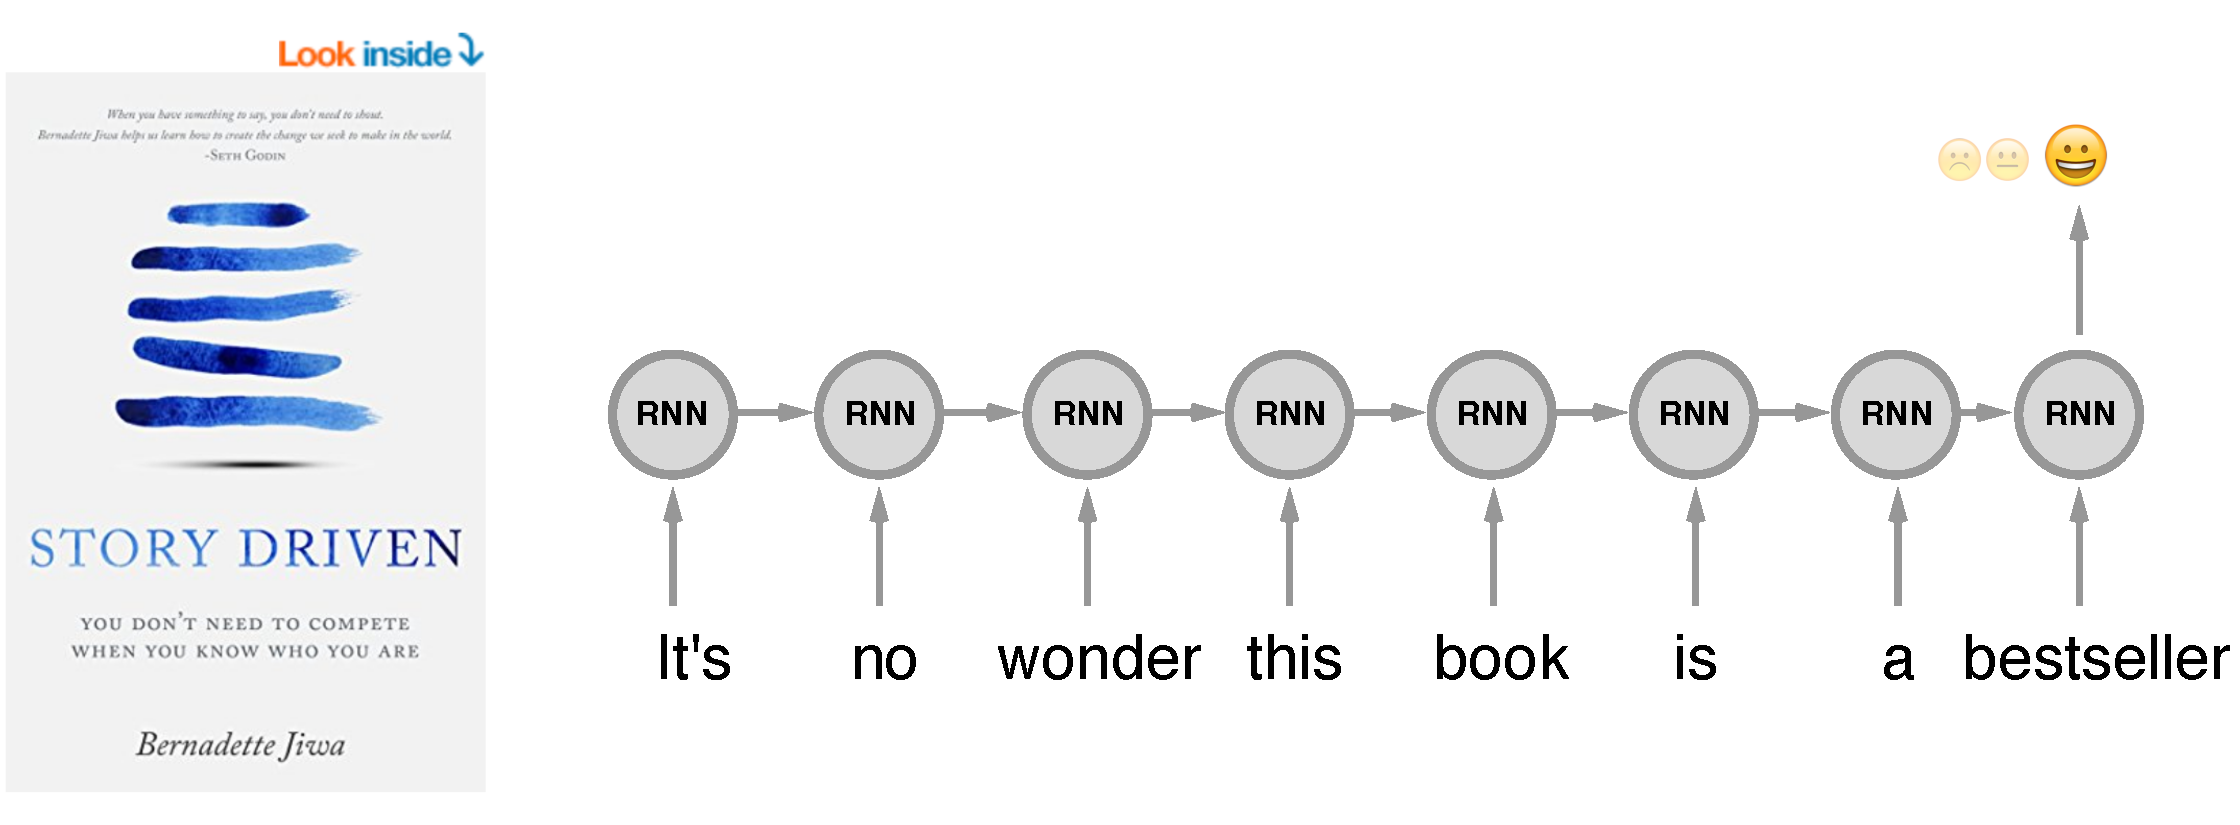
\includegraphics [width=0.8\textwidth]{figures/sentiment_analysis}
				\caption{Sentiment Analysis}
			\end{figure}
			\vspace*{\fill}
	}

	\only<3>{
		\vspace*{\fill}

		\begin{figure}[h]
			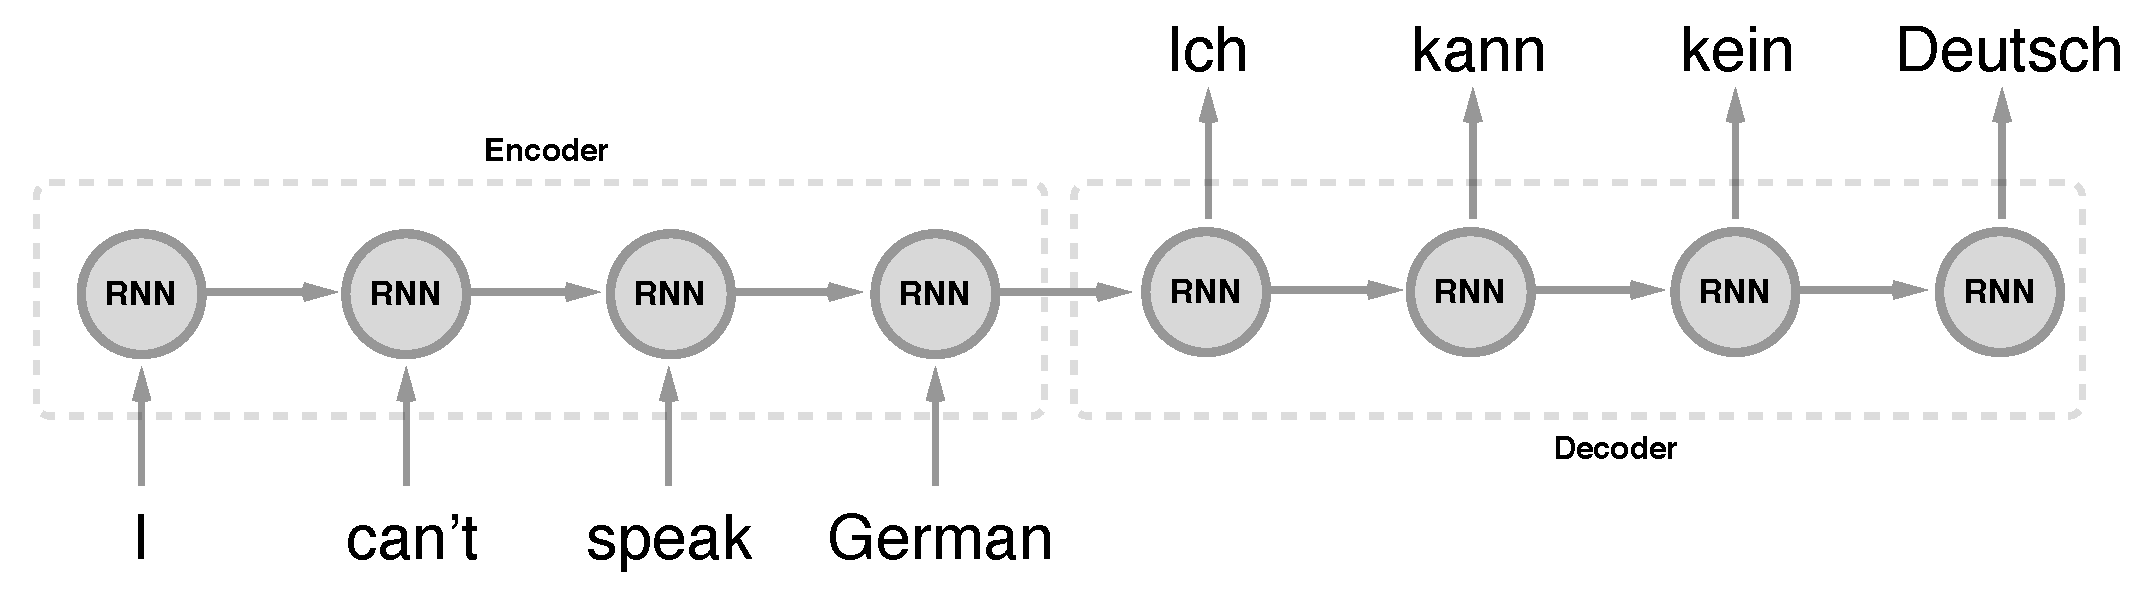
\includegraphics [width=\textwidth]{figures/machine_translation}
			\caption{Machine Translation (seq2seq architecture)}
		\end{figure}
		\vspace*{\fill}

	}
	
	\only<4>{


	\begin{figure}[h]
			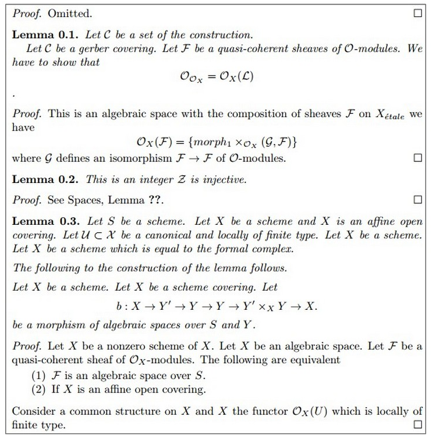
\includegraphics [width=0.4\textwidth]{figures/rnn_effectiveness}
			\caption{An RNN learns to create a \LaTeX \ document.}
			\tiny{\url{http://karpathy.github.io/2015/05/21/rnn-effectiveness/}}
	\end{figure}

	}
}

\end{frame}



\subsection{RNNs from differential equations (Unfolding RNNs)}
\begin{frame}
	\frametitle{Unfolded computations of an RNN}
	\begin{columns}
		\column{0.5\textwidth}
		\only<1>{
		 Assume that $\theta=\{ W^{\text{in}}, W^{\text{rec}} \}$, $\pvec{r}_0 = \pvec{0}$, and the \textbf{forward pass} is constructed as follows:
		 \begin{align*}
		 	\pvec{r}_1 &= W^{\text{in}} \pvec{x}_1 + W^{\text{rec}} \sigma(\pvec{r}_0) \\
		 	&\vdots \\
		 	\pvec{r}_t &= W^{\text{in}} \pvec{x}_t + W^{\text{rec}} \sigma(\pvec{r}_{t-1}) \\
		 	&\vdots \\
			 	\pvec{r}_T &= W^{\text{in}} \pvec{x}_T + W^{\text{rec}} \sigma(\pvec{r}_{T-1}) \\
			\pvec{\hat{y}} &= \pvec{r}_T
		 \end{align*}
		}
		\only<2>{
			\textbf{Backpropagation Through Time} can be derivsed by
			\begin{align*}
				\ppartial{E}{\theta} &= \sum_{k=1}^{T} \ppartial{E}{\pvec{r}_T} \ppartial{\pvec{r}_T}{\pvec{r}_k} \ppartial{^+\pvec{r}_k}{\theta} \\
				\ppartial{\pvec{r}_T}{\pvec{r}_k} &= \prod_{T \ge  i > k} \ppartial{\pvec{r}_i}{\pvec{r}_{i-1}} \\
				&= \prod_{T \ge  i > k} \underbrace{(W^{\text{rec}})^{T}}_{\textbf{!}}  \text{diag}(\sigma'(\pvec{r}_{i-1}))
			\end{align*}
		}
	
		\column{0.5\textwidth}
		 \begin{figure}[h]
				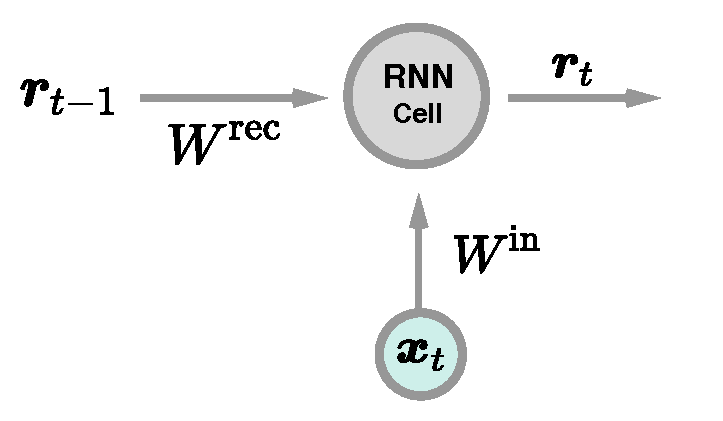
\includegraphics [width=0.8\textwidth]{figures/rnn_computation_example}
			\end{figure}
			\only<2>{
					$\ppartial{^+\pvec{r}_{t+1}}{\theta}$ is the ``immediate" partial derivative. For example, any row in the matrix $\ppartial{^+\pvec{r}_k}{W^{\text{rec}}} $ is $\sigma(\pvec{r}_t)$ \citep{DBLP:conf/icml/PascanuMB13}.
			}

	\end{columns}

%	\only<1>{
%		
%	}
\end{frame}
\subsection{Statistics of RNNs}

\section{Exploding and Varnishing Gradient Problems}
\begin{frame}{Exploding and Varnishing Gradient Problems}
	\begin{itemize}
		\item<1->  The exponential term of $W^{\text{rec}}$ will dominate the calculation of $\ppartial{E}{\theta}$. 
		\item<1-> Two problems can happen:
			\begin{itemize}
				\item Exploding gradient ($\|\nabla_{\pvec{\theta}}E\| \rightarrow \infty $)  
				\item Varnishing gradient ($\|\nabla_{\pvec{\theta}}E\| \rightarrow 0 $)  
			\end{itemize}
		\item<1-> The situation is determined by \textbf{spectral radius} of the matrix $\rho(W^{\text{rec}})$.
				\begin{itemize}
					\item \textit{Spectral radius} of a matrix is its largest absolute eigenvalue.
				\end{itemize}
	\end{itemize}
\end{frame}

\begin{frame}[label=explodinggradient]
\frametitle{Exploding Gradient}

\only<1>{
\begin{itemize}
	\item happens when $\rho(W^{\text{rec}}) > 1$ (for linear cases).
	\item[]
			 \begin{figure}[h]
				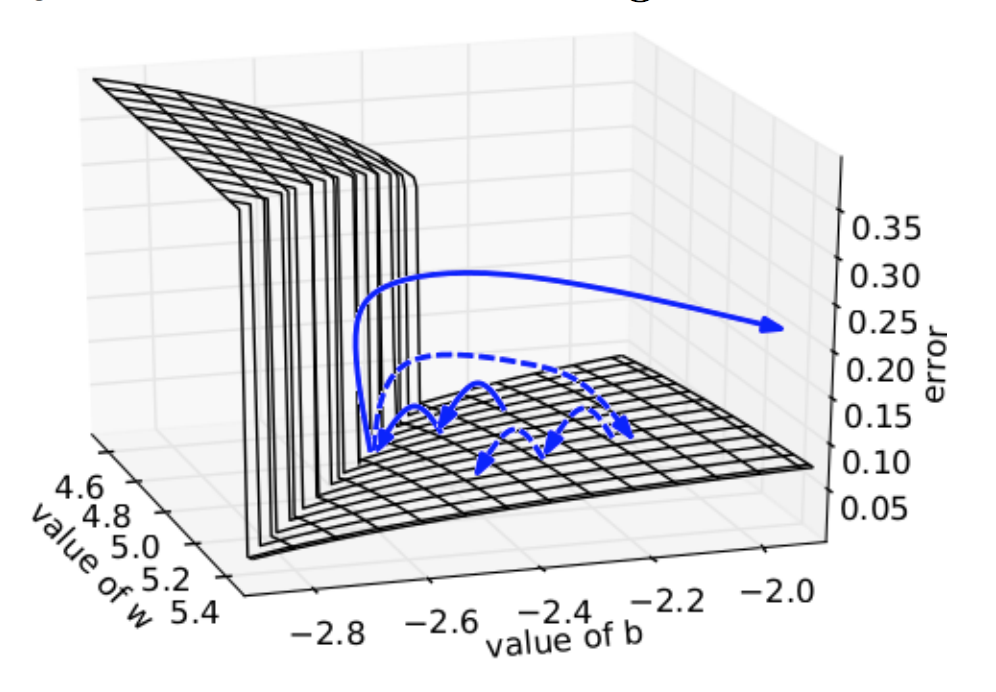
\includegraphics [width=0.4\textwidth]{figures/exploding_gradient}
				\caption{Error Function \citep{DBLP:conf/icml/PascanuMB13}.}
			\end{figure}
	\item causes training \textit{unstable}.
\end{itemize}

}

\only<2>{
Exploding gradient can be alleviated by \textbf{clipping} the norm of the gradient.
			\vspace*{\fill}
				\begin{columns}
						\column{0.5\textwidth}
						\begin{algorithm}[H]
												 \caption{Gradient Clipping \citep{DBLP:conf/icml/PascanuMB13}.}

						 $\epsilon \leftarrow threshold$ \;
						 $\pvec{\hat{g}} \leftarrow \nabla_{\pvec{\theta}} J$\;
				
						  \If{$\|\pvec{\hat{g}}\| \ge threshold $}{
							 $\pvec{\hat{g}} \leftarrow \frac{\epsilon}{\|\pvec{\hat{g}}\|} \pvec{\hat{g}}$;		  	
						   }
						   
					\end{algorithm}
				\end{columns}
			\vspace*{\fill}
}
\end{frame}

%\againframe<2>{explodinggradient}


\begin{frame}[label=varnishing_gradient]
\frametitle{Varnishing Gradient}
\begin{itemize}
	\item happens when $\rho(W^{\text{rec}}) < 1$.
	\item causes RNNs to learn long-term dependencies with a slow progress.
	\item \textbf{Solutions}
		\begin{itemize}
			\item Echo State Networks (ESNs)
			\item Momentum Technique
			\item Long Short-Term Memory Networks
		\end{itemize}
\end{itemize}
	
\end{frame}

\subsection{Echo State Networks (ESNs) }
\begin{frame}[label=esn]
\frametitle{Echo State Networks \cite{JaegerESN}}
	\begin{columns}
		\column{0.5\textwidth}
%			\only<1>{
%
%			}
			\only<1>{
			
			The idea of ESNs is to create a large random reservoir RNN ($W^{\text{rec}}, W^{\text{in}}$). The matrix $W^{\text{rec}}$ is carefully constructed such that reservoir can keep signal \textbf{echoed} in the network for long time.
			
						\begin{align*}
					\tilde{\pvec{h}}_t &= \tanh(W^{\text{in}}\pvec{x}_t+W^{\text{rec}}\pvec{h}_{t-1}), \\
					\pvec{h}_t &= (1-\alpha)\pvec{h}_{t-1} + \alpha \tilde{\pvec{h}}_t, \\
					\hat{\pvec{y}}_t &= W^{\text{out}}\text{concat}(\pvec{x}_t, \pvec{h}_t),
				\end{align*}
				where $W^{\text{rec}} \in \mathbb{R}^{M \times M}$ with $M$ is the number of reservior units, and $\alpha \in (0, 1]$ is the leaking rate.
			
			}
			\only<2> {
			To have the echo state property, the $W^{\text{rec}}$ is typically initialized as 
				\begin{align*}
				W^{\text{rec}} \leftarrow \frac{\xi}{\rho(W^{\text{rec}}) }W^{\text{rec}},
				\end{align*}
				where $\xi$ is a hyperparameter.
			}
			\only<3>{
			ESNs can be viewed as a kernel trick mapping input to a high-dimensional space and learn a linear classifier ($W^{\text{out}}$) there.
			}
		
		\column{0.5\textwidth}
			\vspace*{\fill}
			 \begin{figure}[h]
				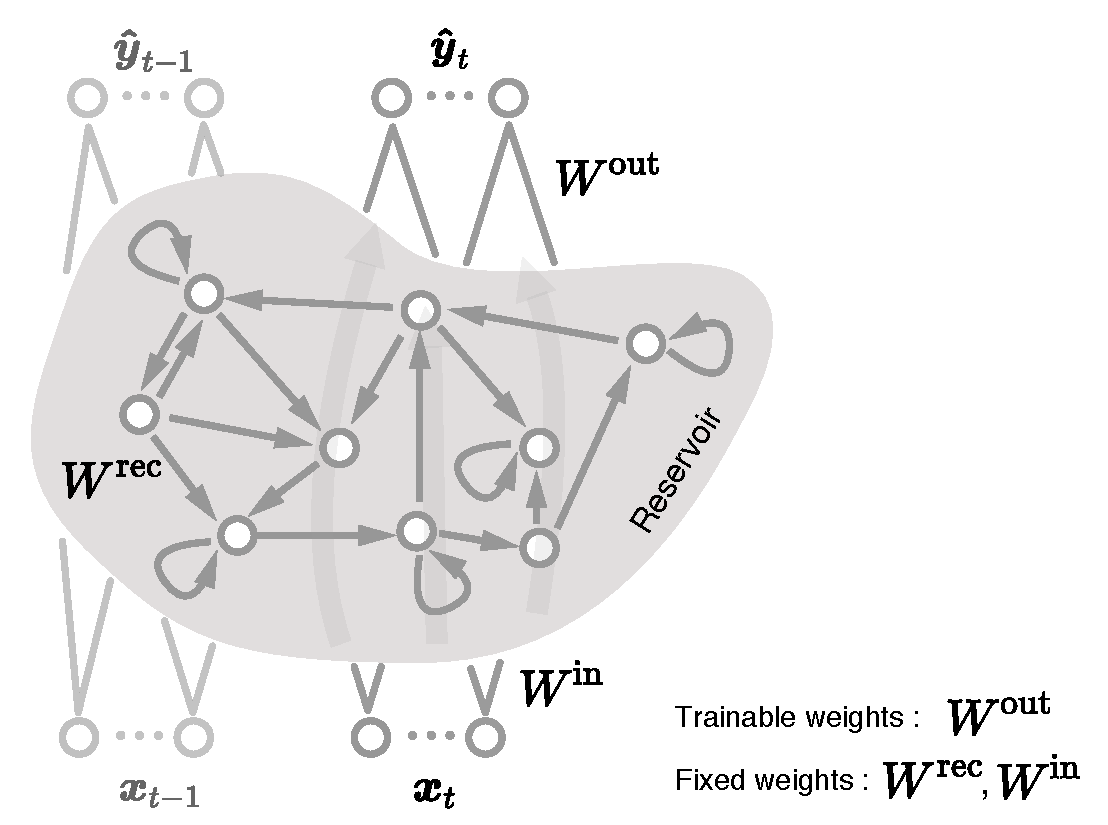
\includegraphics [width=\textwidth]{figures/echo_state_network}
			\end{figure}
			\vspace*{\fill}
	\end{columns}
\end{frame}

\begin{frame}
	\frametitle{An example of the echo state property}
	\only<1>{
			\vspace*{\fill}
			 \begin{figure}[h]
				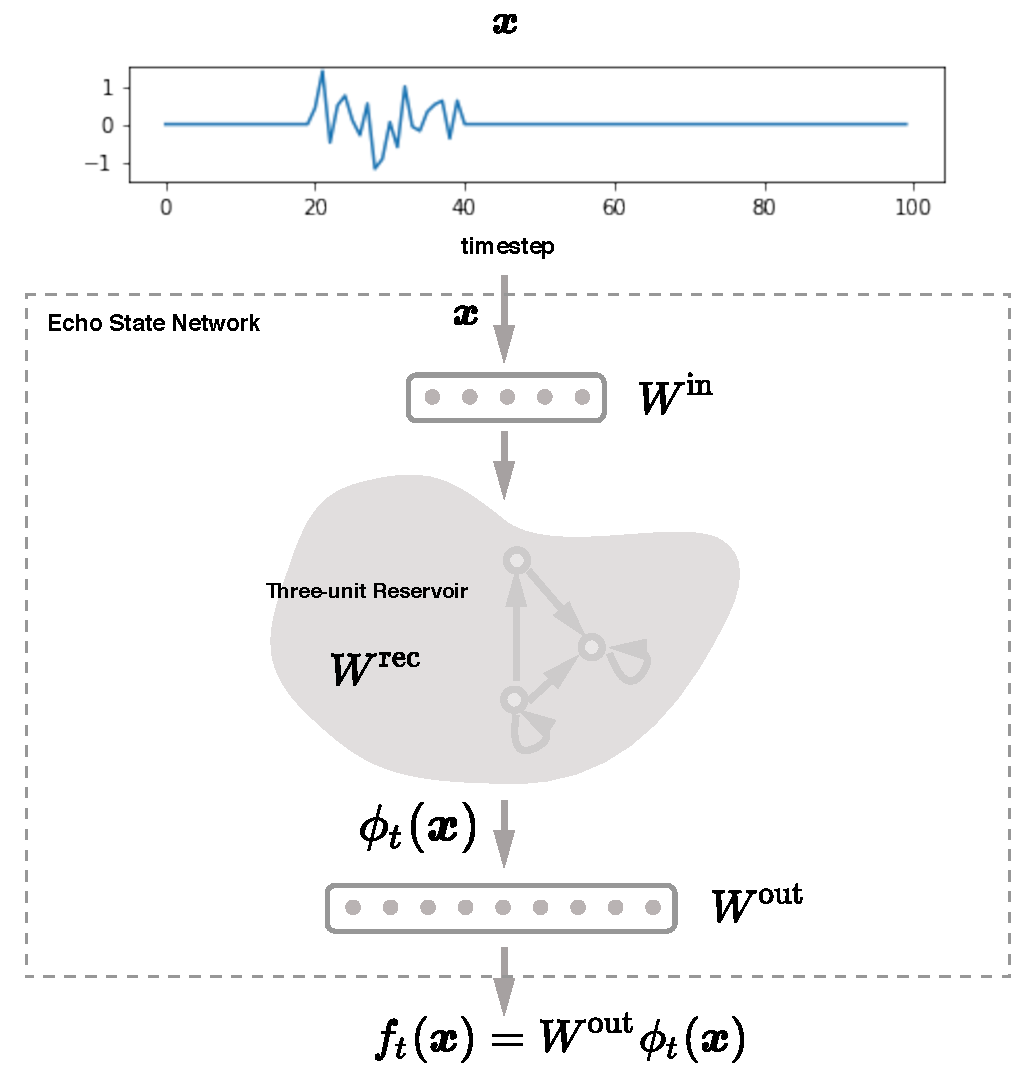
\includegraphics [width=0.45\textwidth]{figures/esn_toyexample}
			\end{figure}
			\vspace*{\fill}
	}
%	\only<2>{
%			\vspace*{\fill}
%			 \begin{figure}[h]
%				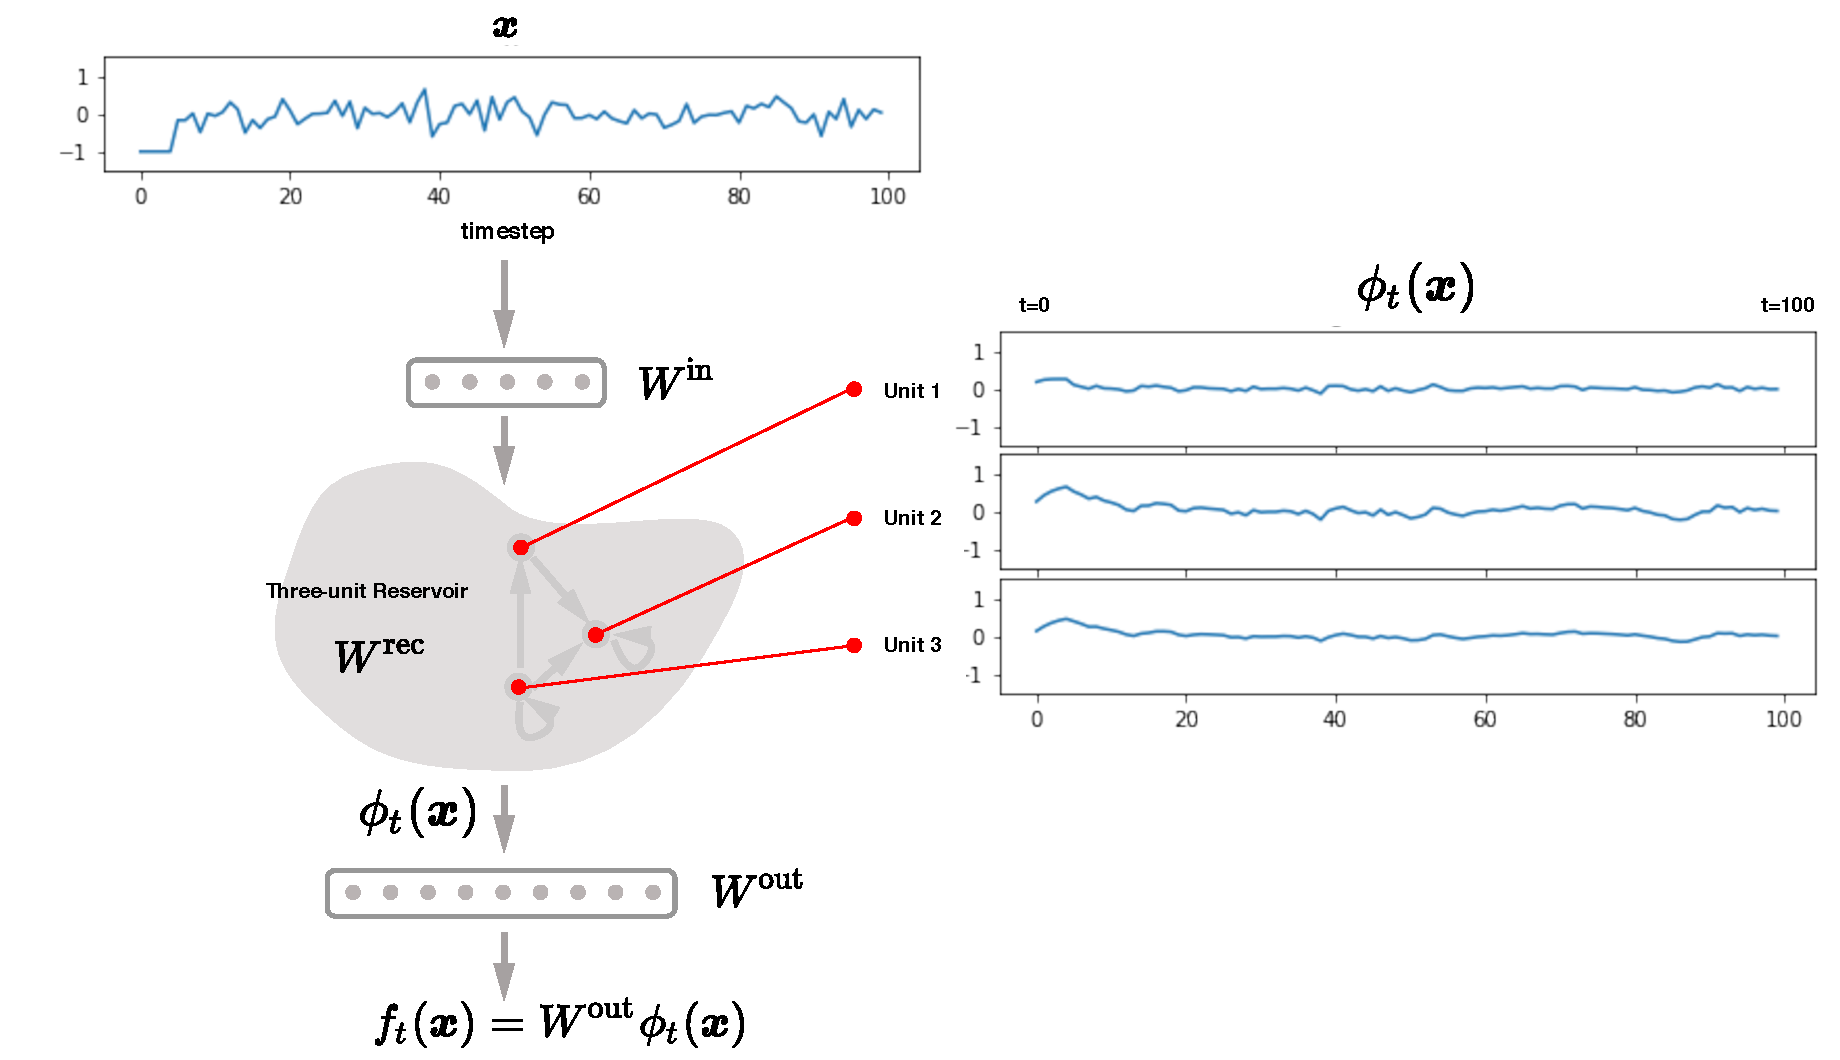
\includegraphics [width=0.8\textwidth]{figures/esn_toyexample_enlarge}
%			\end{figure}
%			\vspace*{\fill}
%	}
	\only<2>{

			An ESN with $\alpha=0.4$ and $\rho(W^{\text{rec}}) = 1.5$.
			\vspace*{\fill}
			 \begin{figure}[h]
				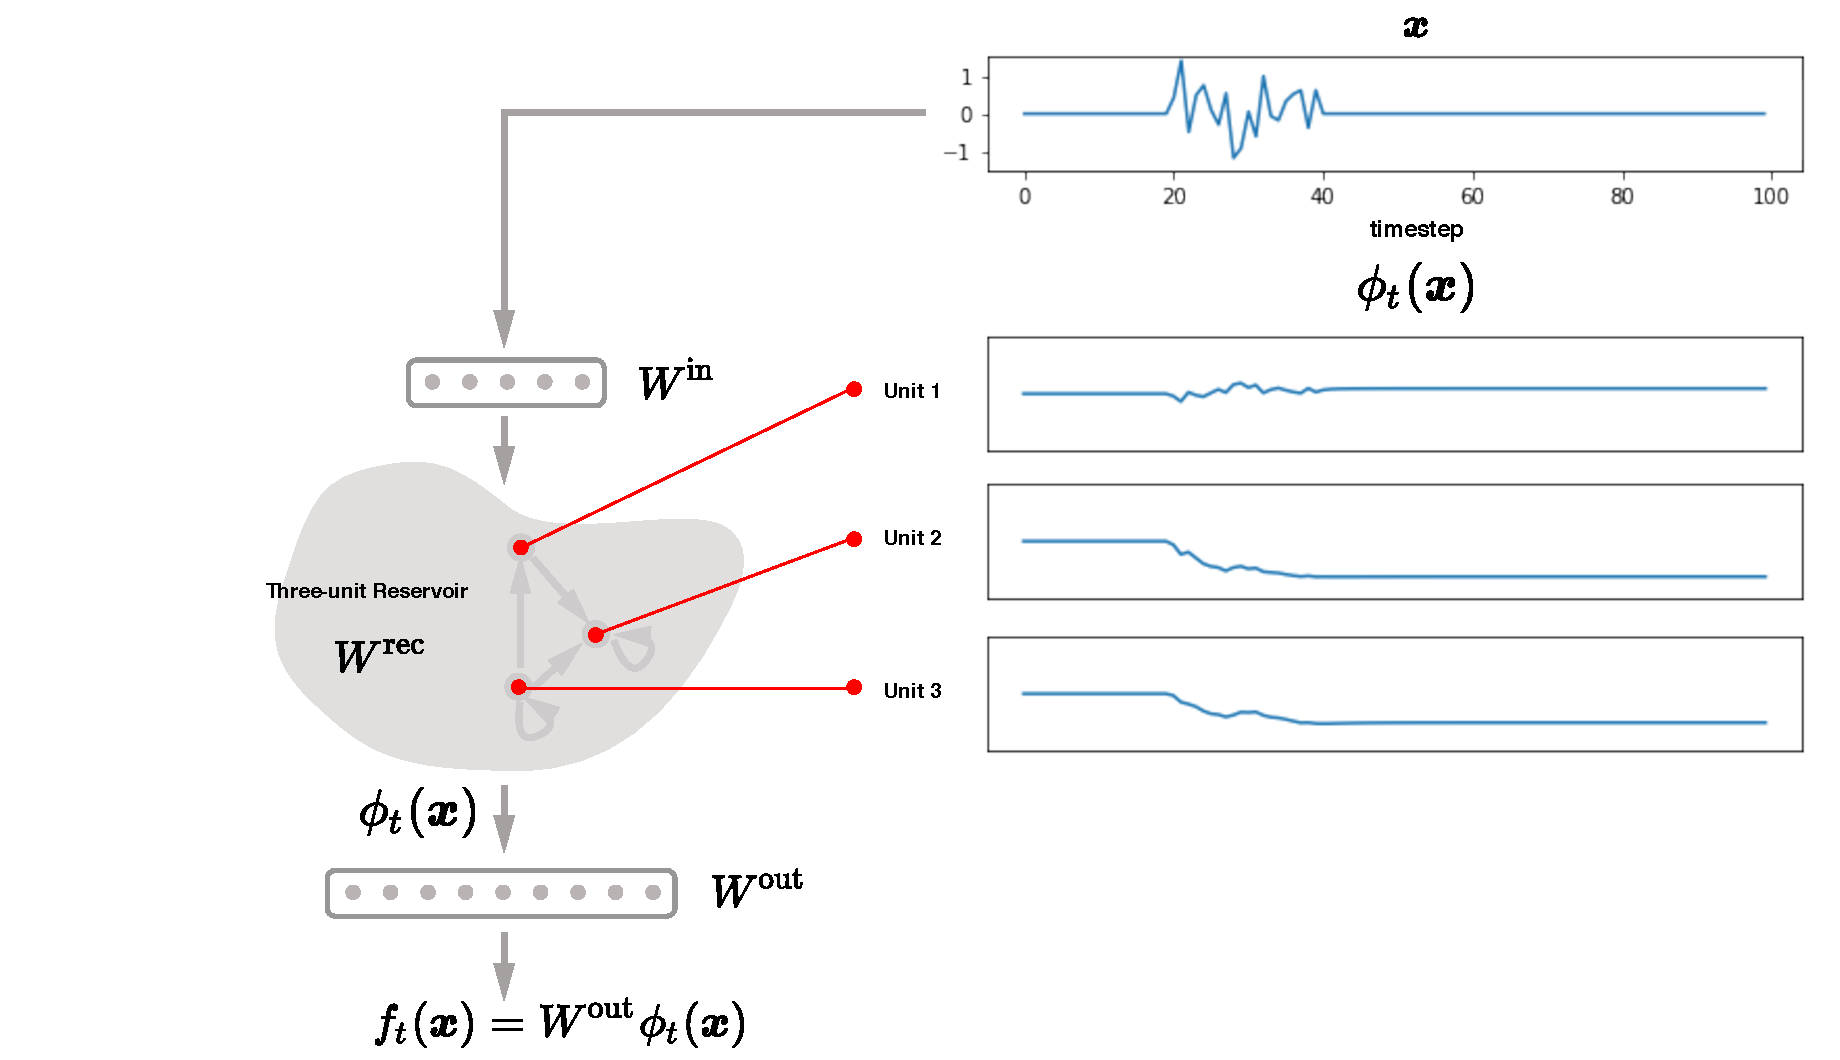
\includegraphics [width=0.8\textwidth]{figures/esn_toyexample_improperly_normalized_wrec}
			\end{figure}
			\vspace*{\fill}
	}
	\only<3>{
		An ESN with $\alpha=0.4$ and $\rho(W^{\text{rec}}) = 0.8$.
			\vspace*{\fill}
			 \begin{figure}[h]
				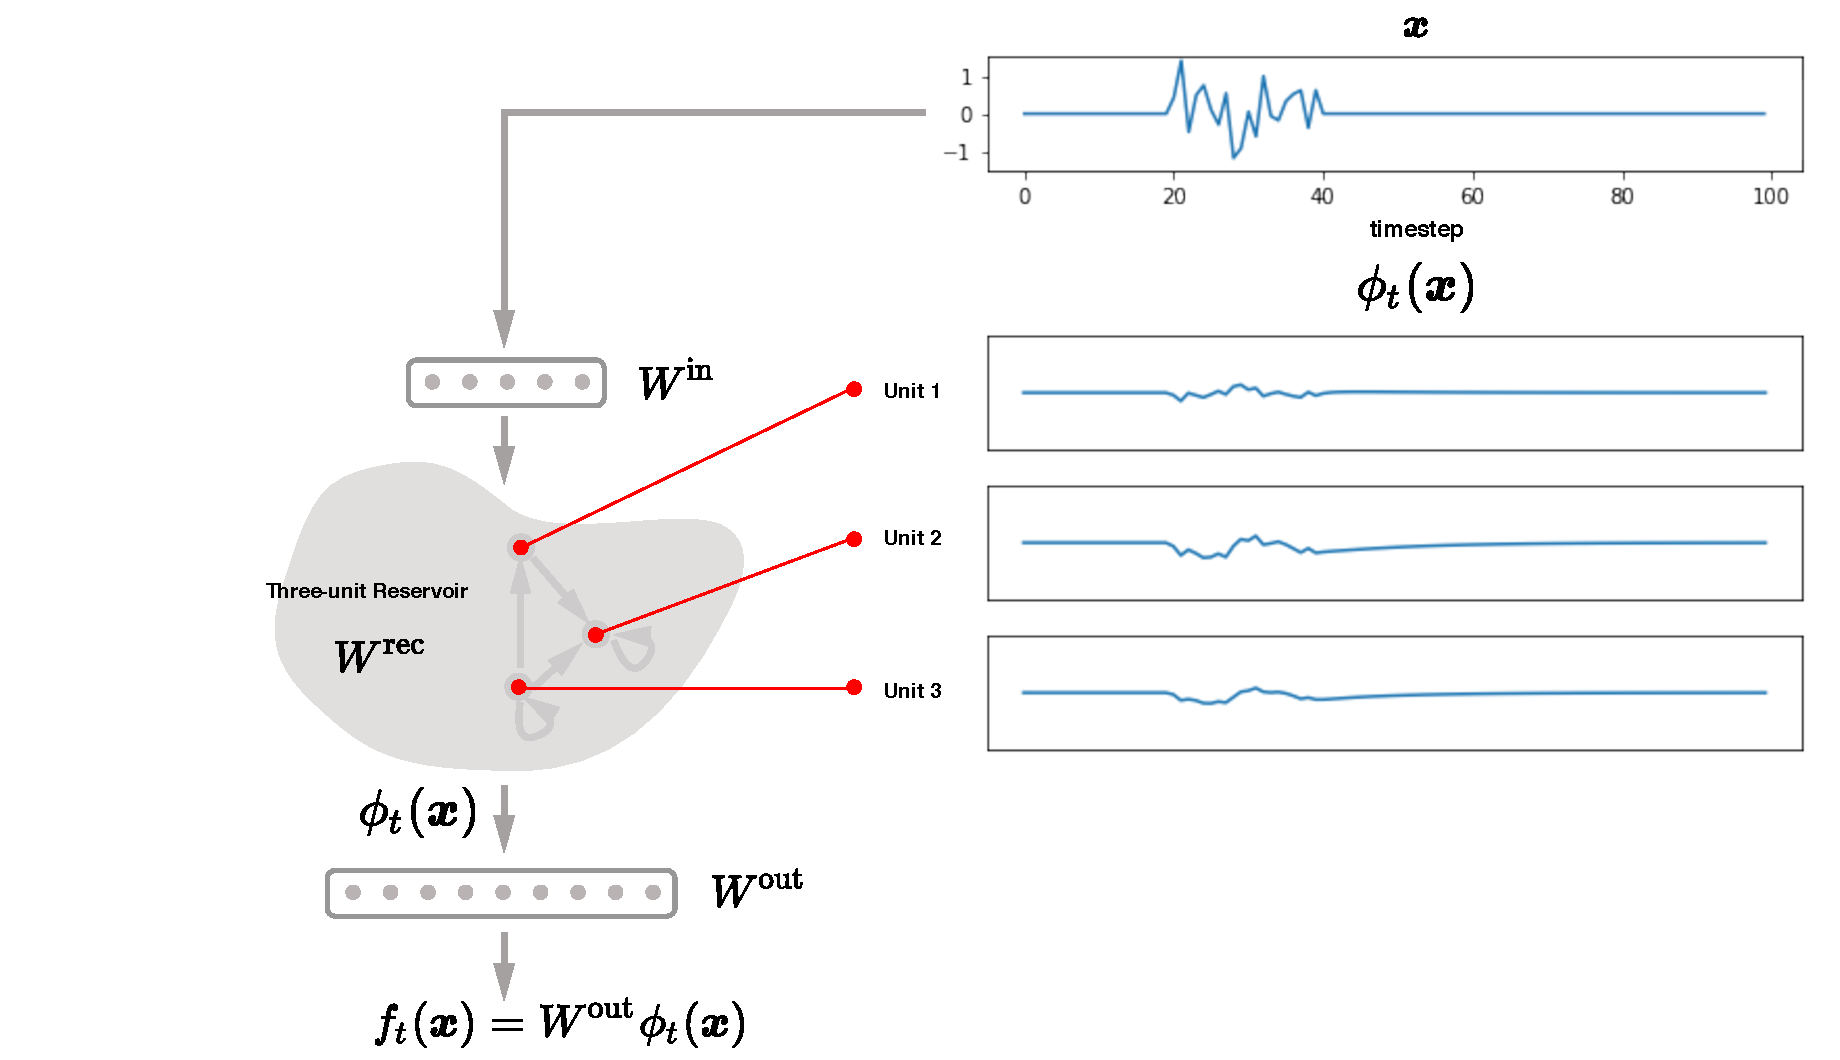
\includegraphics [width=0.8\textwidth]{figures/esn_toyexample_properly_normalized_wrec}
			\end{figure}
			\vspace*{\fill}
	}
		    

\end{frame}

\begin{frame}
	\frametitle{Advantages and Disadvantages of ESNs}
	\begin{columns}
	\column{0.5\textwidth}
		\textbf{Advantages}
					 \begin{itemize}
					 	\item Can be trained very fast.
					 	\item Work well for low dimensional input.
					 \end{itemize}

	\column{0.5\textwidth}	
					 \textbf{Disadvantages}
				 \begin{itemize}
				 	\item Require experiences to initialize $W^{\text{rec}}$ sensibly.
				 	\item Require a big reservoir to solve complex problems.
				 \end{itemize}	

	\end{columns}				
\end{frame}

%
%\subsection{Gradient Descent with Momentum}
%\begin{frame}
%\frametitle{Gradient Descent with Momentum}
%\only<1>{
%\begin{itemize}
%    \item Standard Gradient Descent 
%		$$
%		w \leftarrow w - \lambda \frac{\partial J}{\partial w}
%		$$
%	\item Adam \cite{DBLP:journals/corr/KingmaB14}
%		$$
%		w \leftarrow w - \lambda \frac{\partial J}{\partial w} + someformular
%		$$
%	\item RMSProp \cite{RMSProp}
%\end{itemize}
%}
%\only<2>{
%
%			 \begin{figure}[h]
%				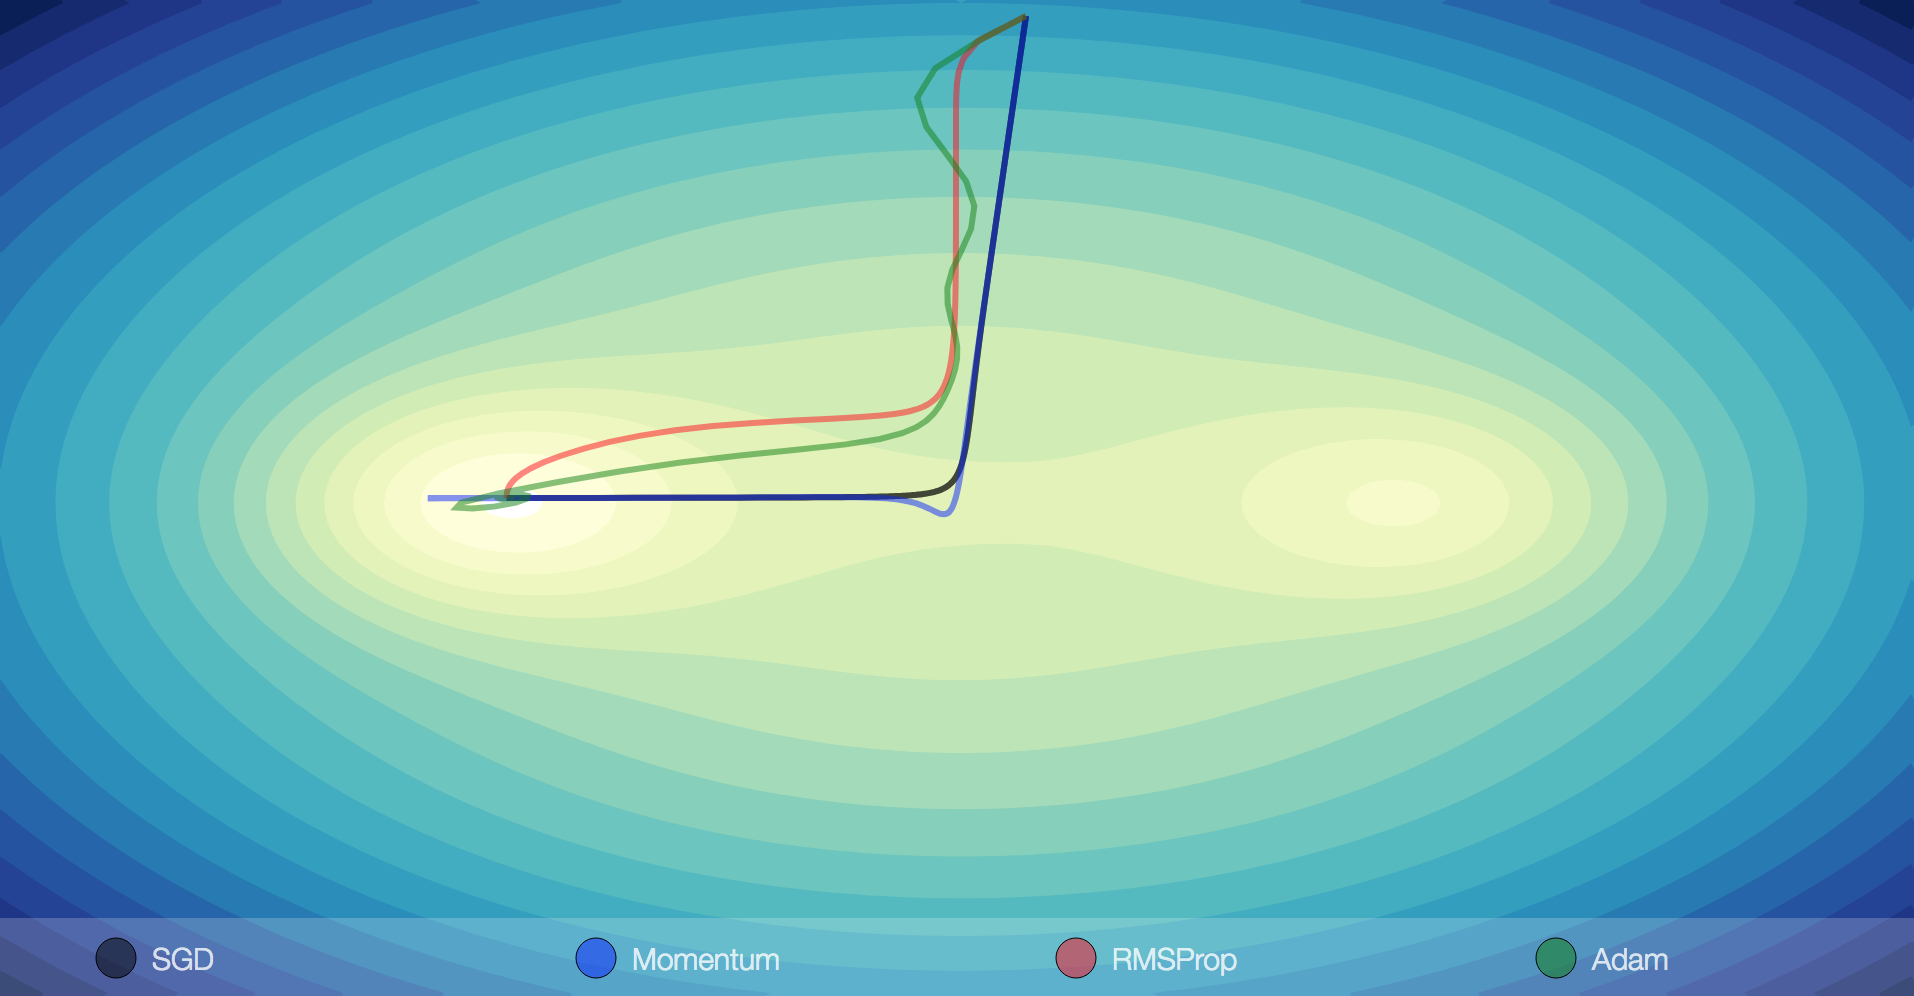
\includegraphics [width=0.5\textwidth]{figures/gradient_methods}
%			\end{figure}
%
%\url{https://cdn.rawgit.com/EmilienDupont/aaf429be5705b219aaaf8d691e27ca87/raw/d5c6bd2483479c8187f5b49e329d84651b930e09/index.html}
%}
%\end{frame}
%\againframe<2>{momentum}

\subsection{Long Short-Term Memory \& Gated RNNs}

\begin{frame}{Long Short-Term Memory (LSTM) \cite{Hochreiter:1997:LSM:265493.264179}}
\begin{columns}
\column{0.5\textwidth}
\begin{itemize}
	\item<1-> Use gating mechanisms and additive updates for $\pvec{c}_t$.
		\begin{itemize}
			\item Eliminate exponential decay factors in the gradient computation
		\end{itemize}
	\item<2-> Employ 3 gates:
		\begin{itemize}
			\item Input gate $\pvec{i}_g$
			\item Forget gate $\pvec{f}_g$
			\item Output gate $\pvec{o}_g$
		\end{itemize}
\end{itemize}
 \column{0.5\textwidth}
 \begin{figure}[h]
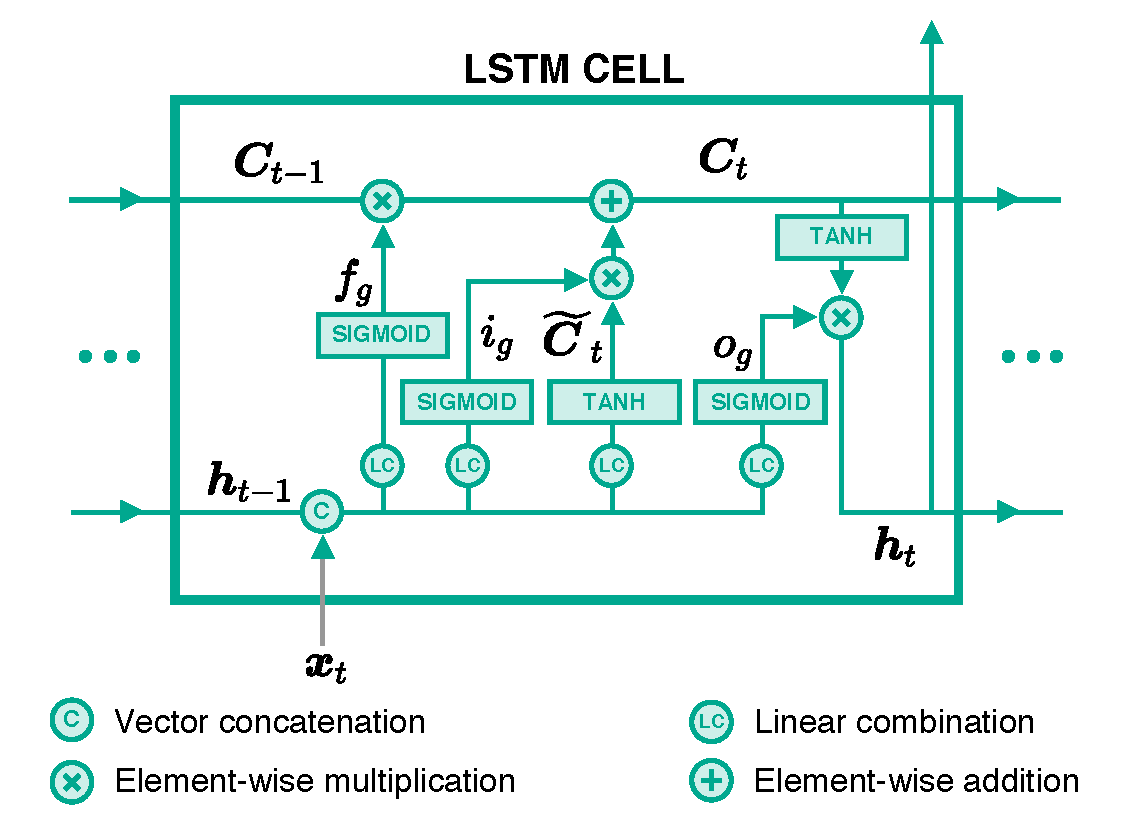
\includegraphics [width=\textwidth]{figures/lstm}
\end{figure}

\end{columns}

\end{frame}

\begin{frame}[label=lstm]
\frametitle{Computations in an LSTM cell}
	\only<1>{
		\begin{columns}
		\column{0.5\textwidth}
		\begin{figure}[h]
		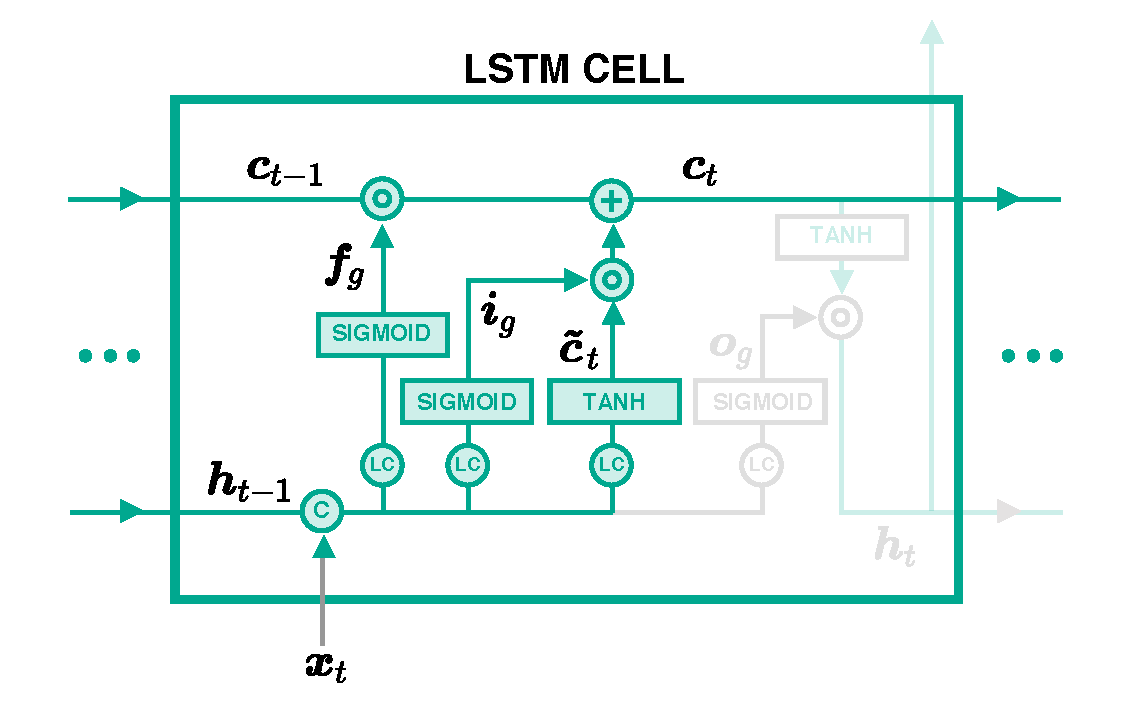
\includegraphics [width=\textwidth]{figures/lstm_input_forget_gate}
		\end{figure}
		 \column{0.5\textwidth}
		\begin{align*}
			\pvec{f}_g &= \textrm{sigm}(U^{(f)} \pvec{x}_t + V^{(f)} \pvec{h}_{t-1})\\
			\pvec{i}_g &= \textrm{sigm}(U^{(i)} \pvec{x}_t + V^{(i)} \pvec{h}_{t-1})\\
			\pvec{\tilde{c}}_t &= \textrm{tanh}(U^{(c)} \pvec{x}_t + V^{(c)} \pvec{h}_{t-1})\\
			\pvec{c}_t &= \pvec{f}_g \circ \pvec{c}_{t-1}  + \pvec{i}_g \circ \pvec{\tilde{c}}_t
		\end{align*}
		\end{columns}	
	}
	
	\only<2>{
			\begin{columns}
		\column{0.5\textwidth}
		\begin{figure}[h]
		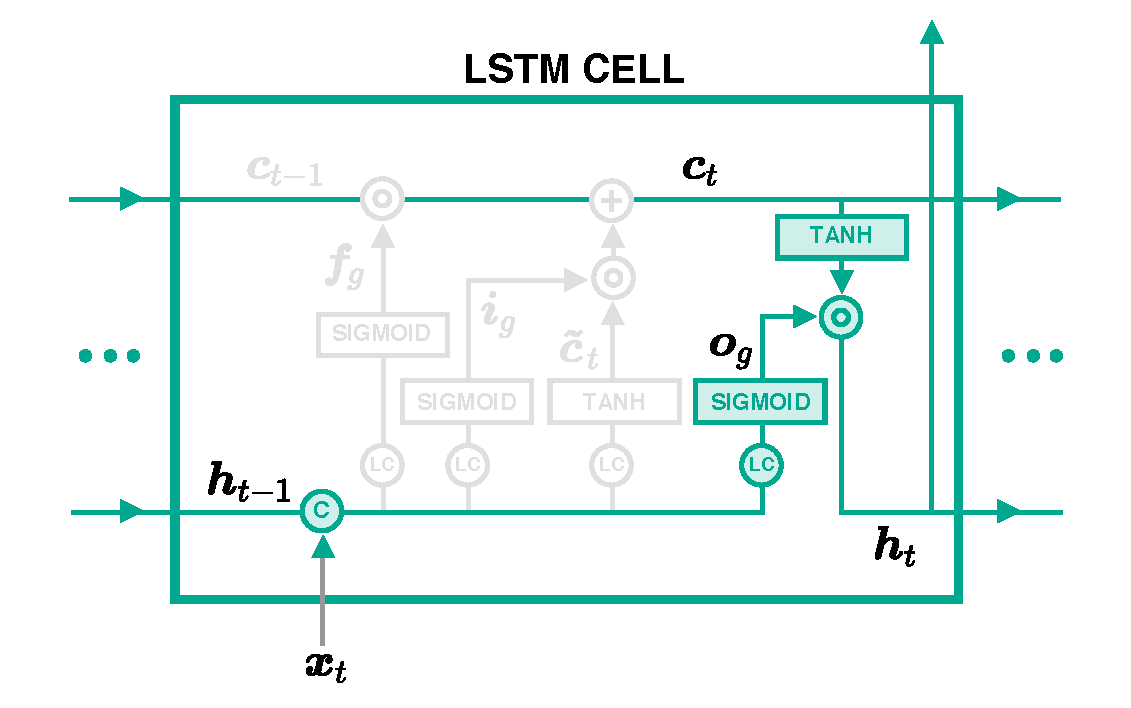
\includegraphics [width=\textwidth]{figures/lstm_output_gate}
		\end{figure}
		 \column{0.5\textwidth}
		\begin{align*}
			\pvec{o}_g &= \textrm{sigm}(U^{(o)} \pvec{x}_t + V^{(o)} \pvec{h}_{t-1})\\
			\pvec{h}_t &= \pvec{o}_g \circ \textrm{tanh}(\pvec{c}_t)
		\end{align*}
		\end{columns}
	}
\end{frame}

\begin{frame}[label=deep_rnn]
\frametitle{Deep RNNs}
%	\begin{enumerate}
		\only<1>{- An RNN for image  segmentation \citep{DBLP:journals/corr/abs-1711-10151}.
				\begin{figure}[h]
					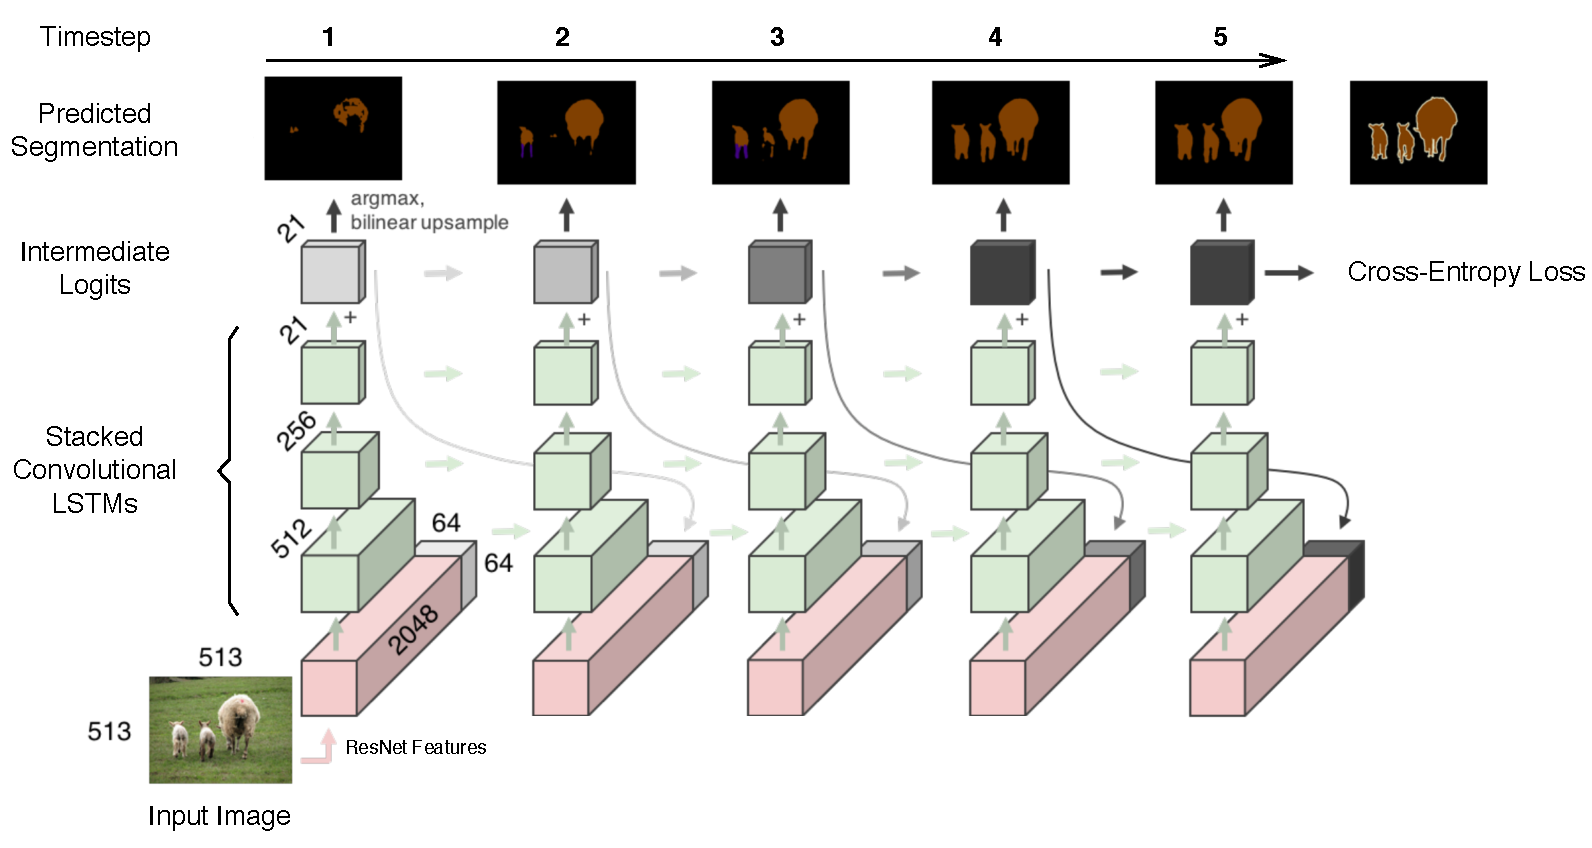
\includegraphics [width=0.8\textwidth]{figures/recurrent_segmentation}
				\end{figure}
		}
		\only<2-4>{- Google's Neural Machine Translation System \citep{DBLP:journals/corr/WuSCLNMKCGMKSJL16}.
			\only<2>{
				\begin{figure}[h]
					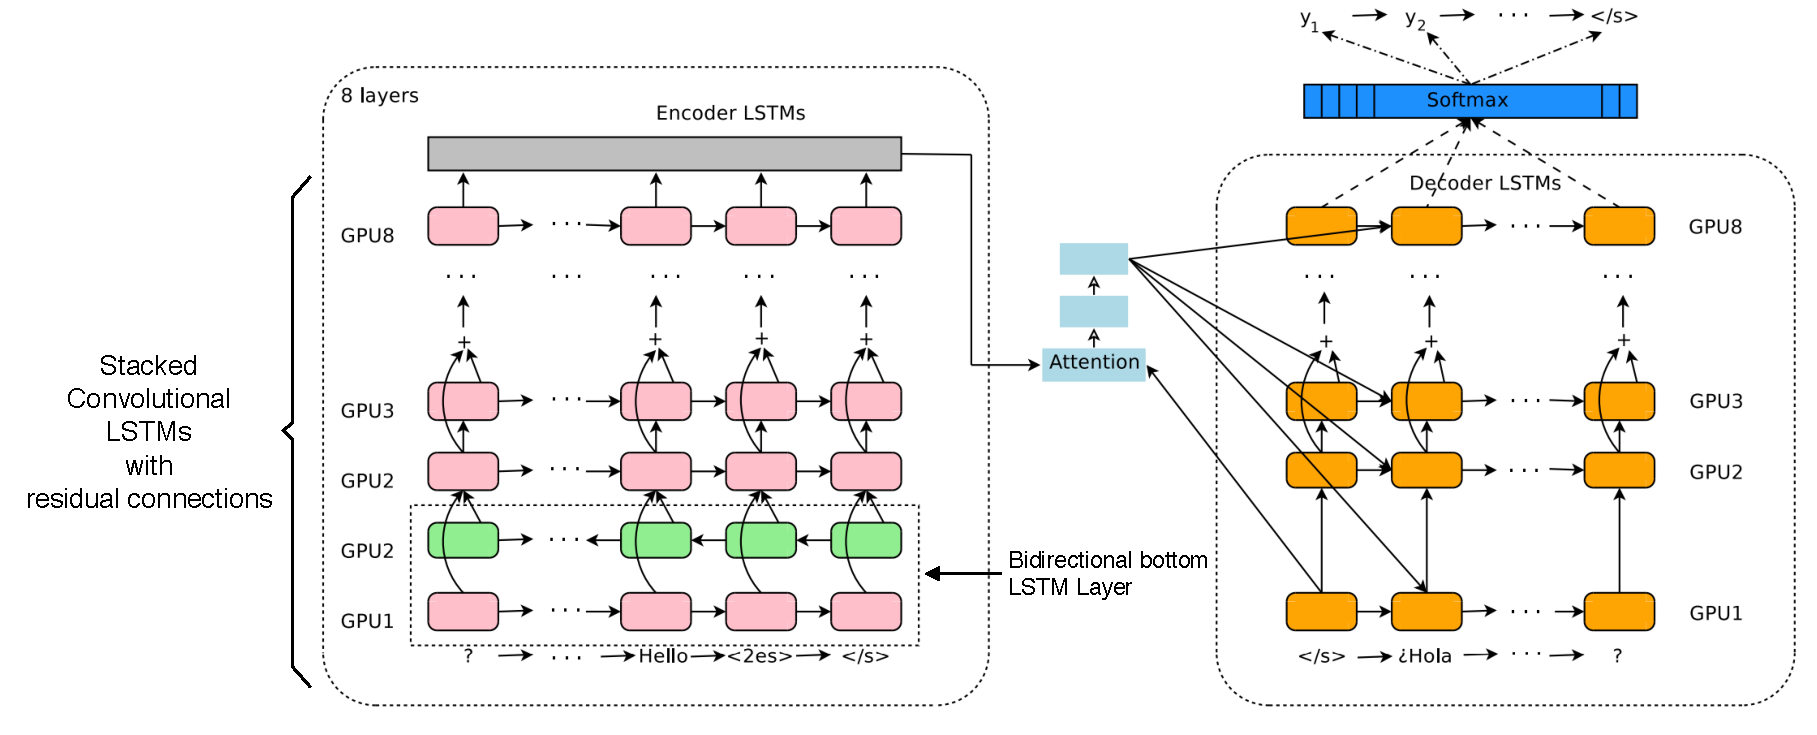
\includegraphics [width=\textwidth]{figures/gnmt}
				\end{figure}
			}
			\only<3>{
				\begin{figure}[h]
					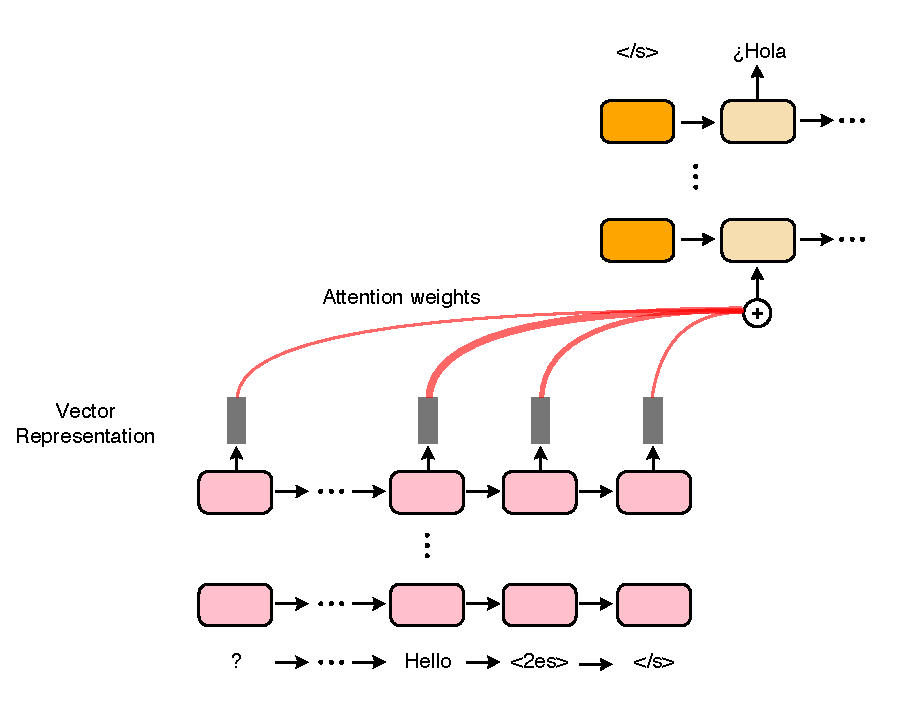
\includegraphics [width=0.7\textwidth]{figures/gnmt_attention}
				\end{figure}
			}
			\only<4>{
				\\ \vspace{0.5cm} \hspace{1cm} $\forall t, 1 \le t \le M $
				\begin{align*}
							s_t &= \text{AttentionFunction}(\boldsymbol{y}_{i-1}, \hat{\boldsymbol{x}}_t) \\
							p_t &= \text{exp}(s_t)/ \sum_{t=1}^{M} \text{exp}(s_t) \\
							\boldsymbol{a}_i &= \sum_{t=1}^M p_t \hat{\boldsymbol{x}}_t
				\end{align*}
				where 
				\begin{itemize}
					\item $M$ is a number of tokens in the sequence.
					\item \textit{AttentionFunction} can be implemented using a feed forward neural network.
				\end{itemize}

			}
		}
		

\end{frame}




\begin{frame}[allowframebreaks]
        \frametitle{References}
        \bibliographystyle{amsalpha}
        \bibliography{reference.bib}
\end{frame}
\end{document}
